\section{Solving the multi-objective WSN problem}
\label{section:solution}
As defined in the previous Section, we seek a method to optimise multiple objectives in our WSN system. To do so we will incorporate two algorithms. We give the high-level purpose and requirements of each algorithm in the next sections, however, full details and theoretical justification can be found in \ref{XXX}
\todo[inline]{Reference to preprints? here}

\subsection{Optimisation algorithms for task allocation and resource allocation}
The \acronymATARIAExtended{}{} algorithm will enable agents in the system to learn the best agents to allocate tasks to to obtain the best composite task values, as well as explore the system for other agents, and adapt to impacts and outages. Each agent $\varAgent{}{}$ in the network is required to maintain two main data sets. Firstly, \textit{Q-value mappings} $qm(g, typea(AT^{\ominus}))$, where $typea$ maps each of the unallocated atomic tasks $AT^{\ominus}$ to its type. This is a set of values mapped to actions the agent can take. These are used by the \acronymATARIA{}{} algorithm to select actions based on the learned outcomes of previous actions. Secondly, the set of \textit{action samples}, $\Sigma$, the historical $\functionCompositeTaskValue{}{}$ values collected as the agent completed past composite tasks. Using these inputs the \acronymATARIA{}{} algorithm will learn to select actions that generate the best composite task values, and adapt the choice of action depending on how good the composite task values are in comparison to the historical values.

The \acronymMGRAOExtended{}{} algorithm, helps agents executing measurement tasks allocate their resources to optimise the composite task value as well. For this algorithm each agent maintains a matrix of values, $PW_{cg,r}$ , the \textit{resource allocation weights matrix}, that maps the its resources, in this case energy, to the atomic task types it can complete. In addition, there is the The \textit{eligibility trace matrix}, $E_{cg}$, a set of values that measures how recent each element in the resource weights matrix impacted an atomic task value.


\subsection{Extension to hierarchical task allocation}

To enable agents to form arcs as described we allow atomic tasks to be re-allocated to further agents in order to reach an agent within range of a demand point. Figure \ref{fig:arc-flow} illustrates an arc where there are two re-allocations needed before a specific atomic task is allocated to an agent whose sensor is in range of the demand point, and can therefore make a measurement.

\begin{figure}[ht]
	\centering
	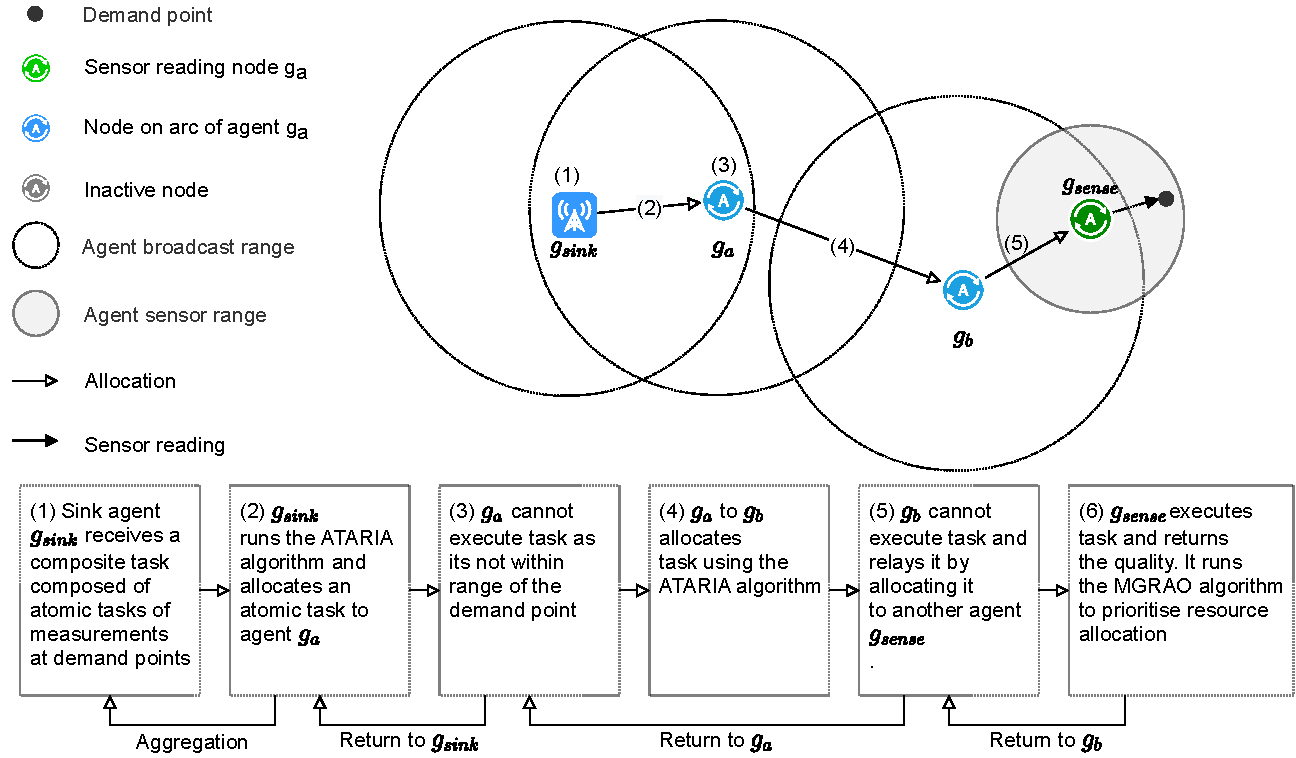
\includegraphics[width=0.9\linewidth]{arc-flow}
	\caption{\textbf{Allocation along an arc}. This diagram illustrates how allocations can be relayed along an arc using successive applications of the \acronymATARIA{}{} algorithm.}
	\label{fig:arc-flow}
\end{figure}

\subsection{Algorithm for optimising hierarchical task allocation in networks of agents}
\todo[inline]{DOesnt really need a name}
The \acronymWSNOptimisationExtended{}{} algorithm is defined in Algorithms \ref{alg:wsn_optimisation_sink}
and \ref{alg:wsn_optimisation_arc}, which are split for clarity. The flowchart in Figure \ref{fig:algorithm-flow} shows how this agents utilise \acronymATARIA{}{} and \acronymMGRAO{}{} with these recursive actions enabled. 

\begin{figure}[ht]
	\centering
\begin{subfigure}{.49\textwidth}
	\centering
	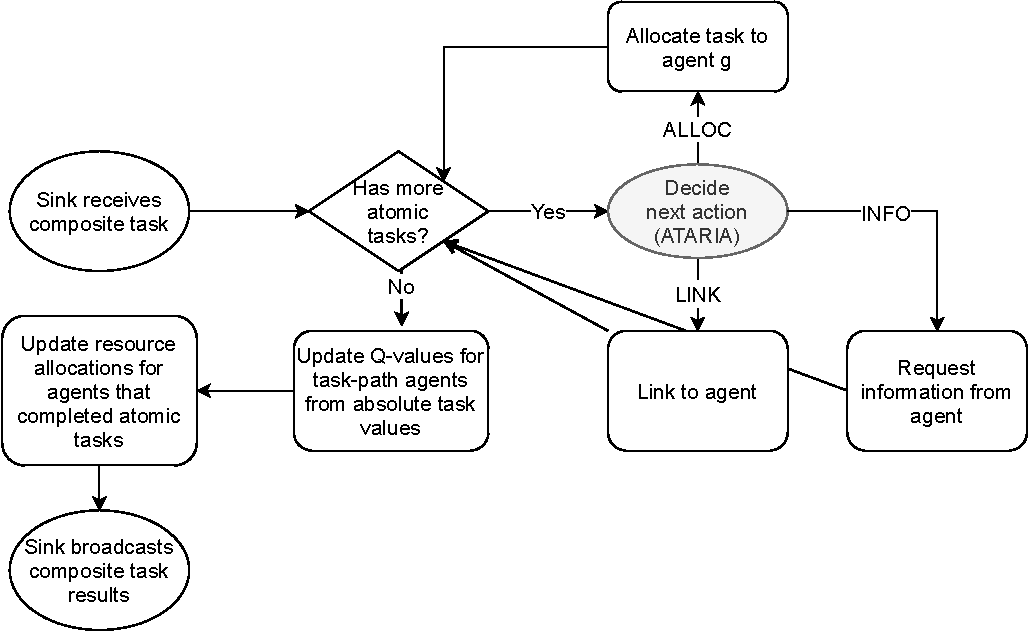
\includegraphics[width=0.9\linewidth]{algorithm-flow-sink}
	\caption{Sink agent flow}
	\label{fig:algorithm-flow-sink}
\end{subfigure}
\begin{subfigure}{.49\textwidth}
	\centering	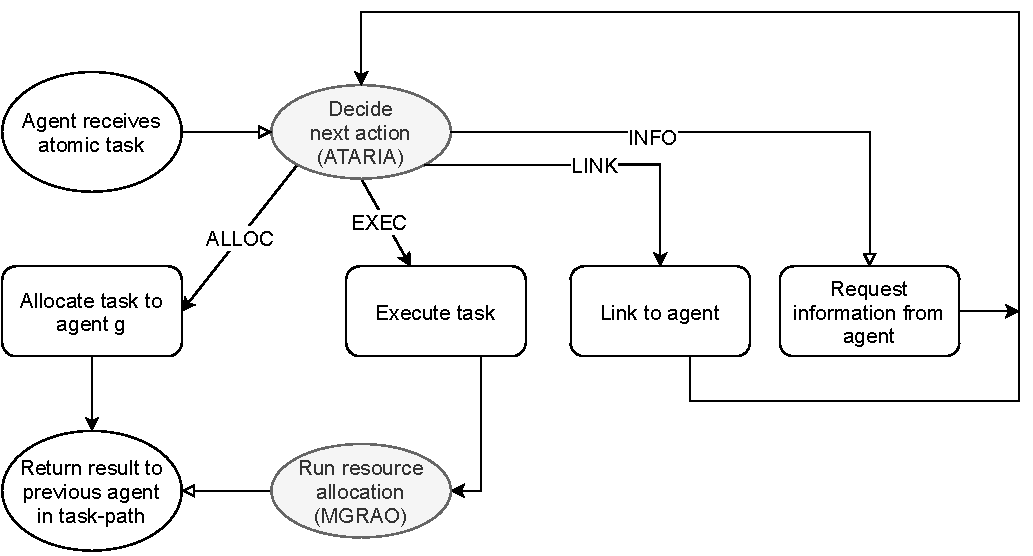
\includegraphics[width=0.9\linewidth]{algorithm-flow-arc}
	\caption{Arc agent flow}
	\label{fig:algorithm-flow-arc}
\end{subfigure}
	\caption{\textbf{\acronymWSNOptimisation{}{}} - Flow chart of combined \acronymATARIA{}{}/\acronymMGRAO{}{} execution. The two algorithms are combined together to allow recursive allocation of tasks and learning of the network.}
\label{fig:algorithm-flow}
\end{figure}